\input{../header}
\hyphenpenalty=5000

\rhead{Your name: \rule{8cm}{0.15mm}}

\begin{document}

\section{Learning target C1, version 3}


\begin{enumerate}[leftmargin=0pt]
		\item  For the function $f$ plotted at left, sketch an accurate graph of its derivative, $f'$, on the axes at right. \\  

\begin{center}  
  \scalebox{0.3}{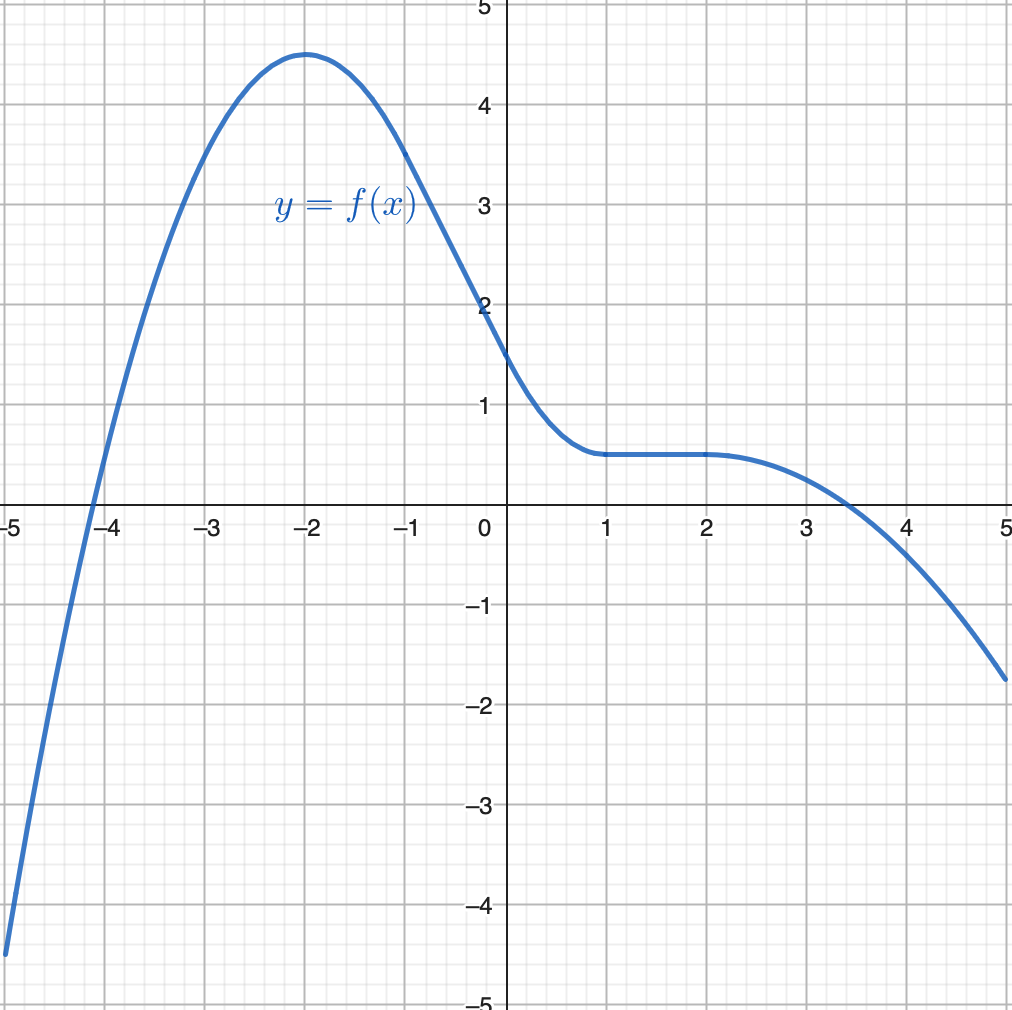
\includegraphics{images/CP-3-LT-1-graph-F23.png}} \hspace{0.25in} \scalebox{0.3}{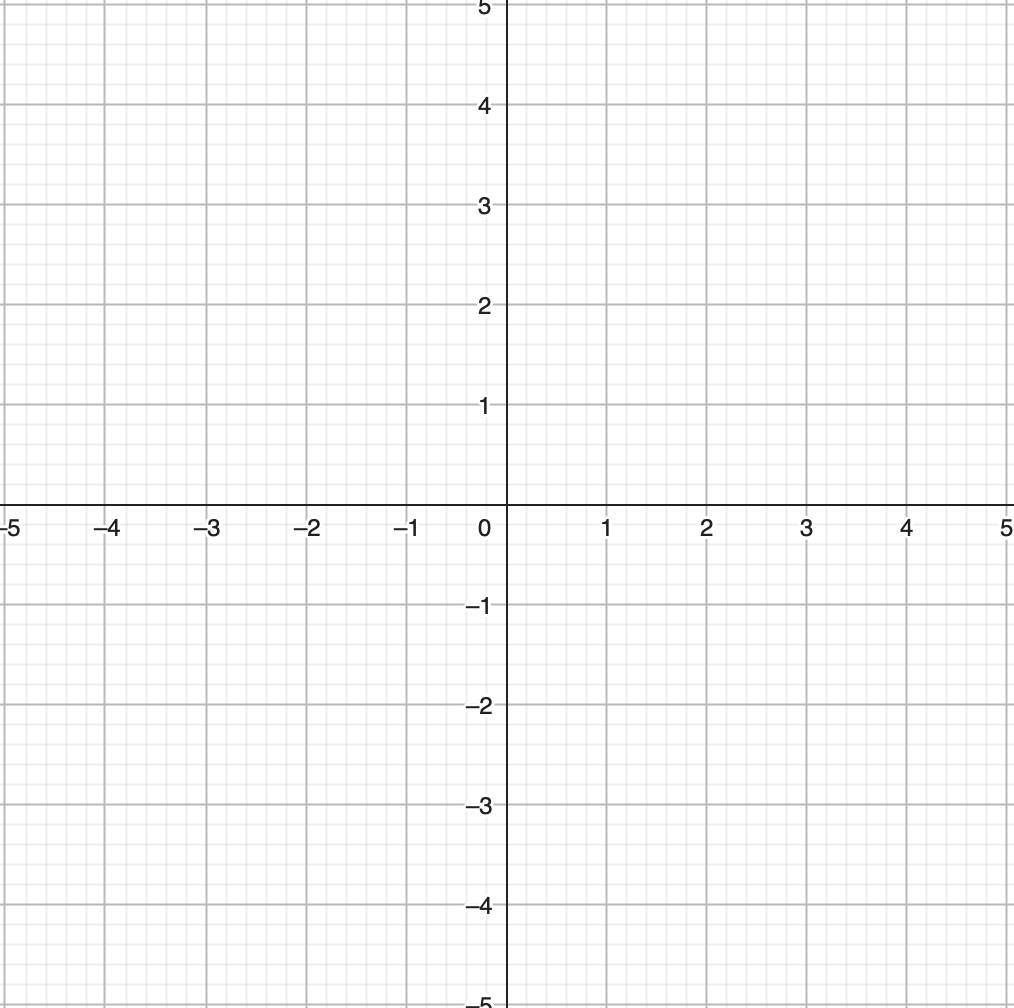
\includegraphics{images/CP-1-LT-1-grid-F23.png}} \\
\end{center}


	\item % Now make this one tabular and with complicated functions
Consider the two piecewise linear functions $r$ and $s$ given by the figure below.  Determine each of the following derivative values that involve functions that are defined in terms of $r$ and $s$.  Clearly show your work and thinking using proper notation, be sure your values are \emph{exact} in light of the given information, and write one sentence to explain your overall approach.
	
\begin{center}  
  \begin{minipage}{0.4\linewidth}
    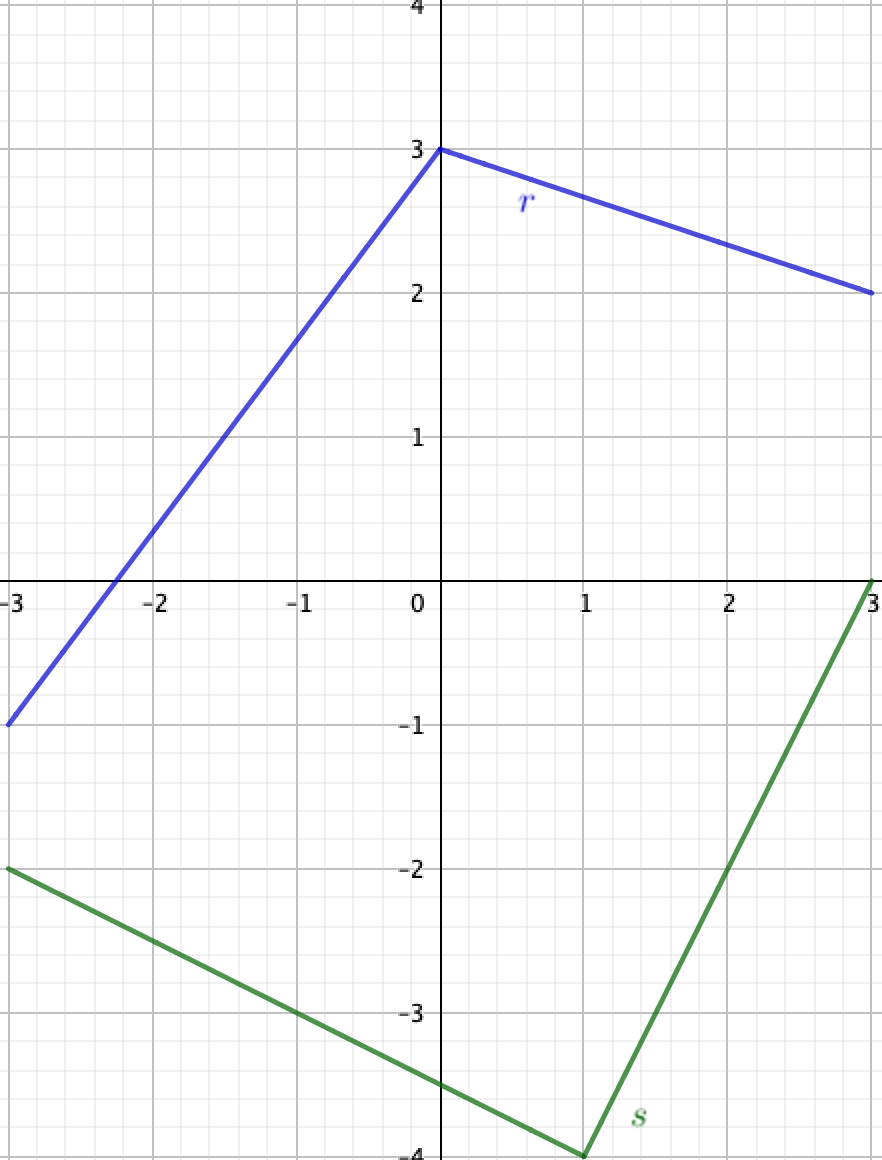
\includegraphics[width=\textwidth]{images/CP7-01-3LTs.png}
  \end{minipage} %
  \begin{minipage}{0.55\linewidth}
    \begin{enumerate}
        \item[(i.)] If $M(x) = s(r(x))$, find $M'(2)$. \\  
        
        \vspace{1in}
        \item[(ii.)] If $T(x) = r(x^3)$, find $T'(-1)$. 
        \vspace{1in}
      \end{enumerate}

\end{minipage}
\end{center}


		\item Evaluate the following definite integral exactly using the Fundamental Theorem of Calculus.  Show your full work and thinking using proper notation.
		
		$\displaystyle \int_{\pi/2}^{\pi} \left(\sin(x) + 2e^x - \frac{1}{x} \right) \, dx$
\end{enumerate}

%%%%%%%%%%%%%%%%%%%%%%%%%%%%%%%%%%%%%%%%%%%%%%%

\pagebreak


%%%%%%%%%%%%%%%%%%%%%%%%%%%%%%%%%%%%%%%%%%%%%%%%%%%%%%%%%%%%%%%%%%

\section{Learning target I1, version 2}
Compute approximations of definite integrals using numerical methods. Decide when each method gives overestimates vs. underestimates.

\hrulefill

Consider the function \(g(x)=\sqrt{1-x^2}\). 

\begin{enumerate}[(a)]
  \item Use Geogebra or Desmos or something to draw a graph of this function.
  \item Based on, like, geometry, what's \(\displaystyle\int_{-1}^1 g(x)\ dx\)? Why?
  \vfill

  \item So then we can figure out a good approximation to \(\pi\) if we figure out a good approxmation to \(\int_{-1}^1 g(x)\ dx\). Use appropriate technology, such as Geogebra or a Riemann sum applet, to approximate this area using left, right, midpoint, and trapezoid sums with 10 subintervals:
  \begin{itemize}
    \item $L_{10}=$
    \item $R_{10}=$
    \item $M_{10}=$
    \item $T_{10}=$
  \end{itemize}
  Report your answers with at least 6 decimal places of accuracy.
  
  \item Which of these approximations are overestimates and which are underestimates? \\
  How can you tell?
  \vfill

  \item Use your calculations from part (b) to approximate \(\displaystyle\int_{-1}^1 g(x)\ dx\) using Simpson's rule.

  \vfill
  \item And lastly but not leastly, give a good approximation of \(\pi\) based on your work.
\end{enumerate}
\pagebreak
%%%%%%%%%%%%%%%%%%%%%%%%%%%%%%%%%%%%%%%%%%%%%%%%%%%%%%%%%%%%%%%%%%

\section{Learning target I2, version 3}

Given appropriate data about a function, determine outputs, direction, and concavity of its \\
antiderivative, and/or construct an accurate graph.

\hrulefill


Consider the piecewise linear function $y = f(x)$ pictured below; assume that $f(x) = 0$ for $x \le -1$ and $f(x) = 1$ for $x \ge 11$.
	
	\begin{center}
		\scalebox{0.35}{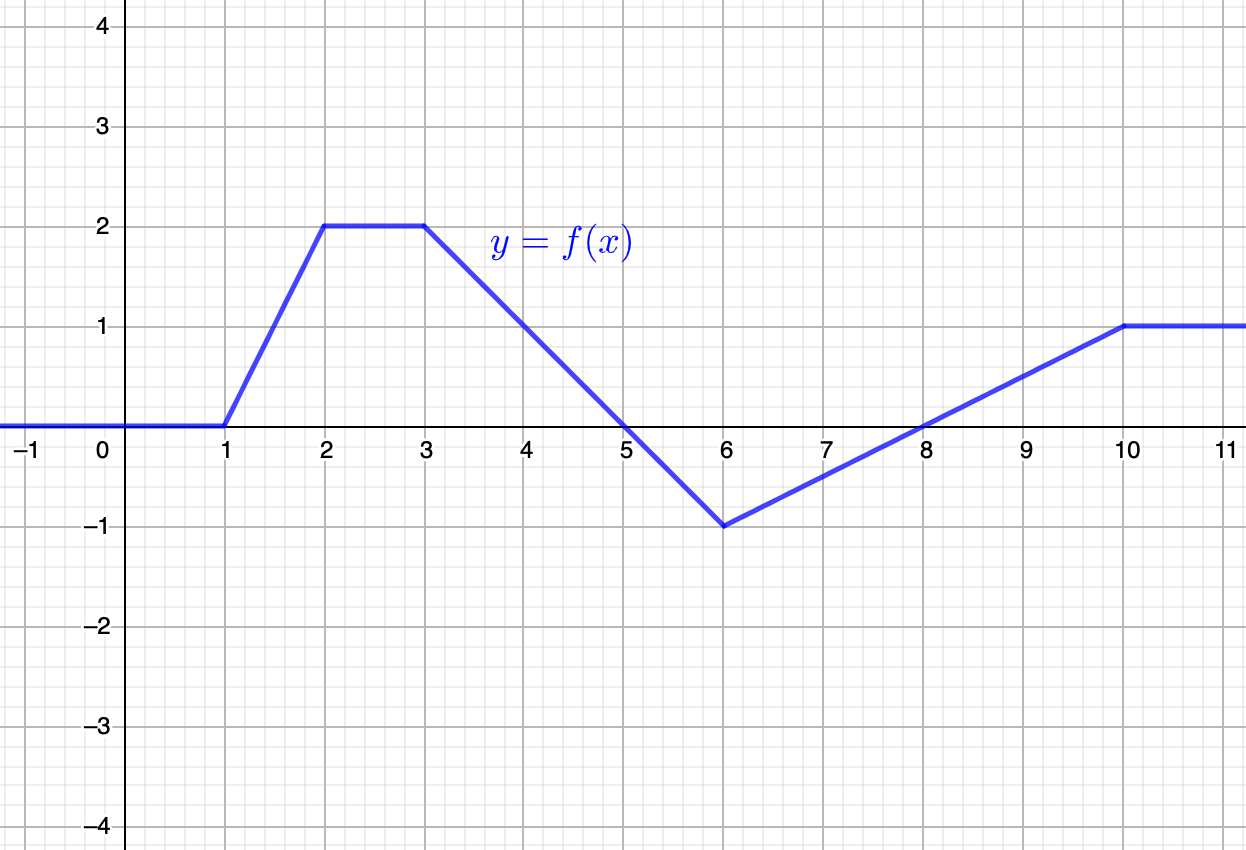
\includegraphics{images/CP-3-LT2-graph.png}} \hspace{0.25in} \scalebox{0.35}{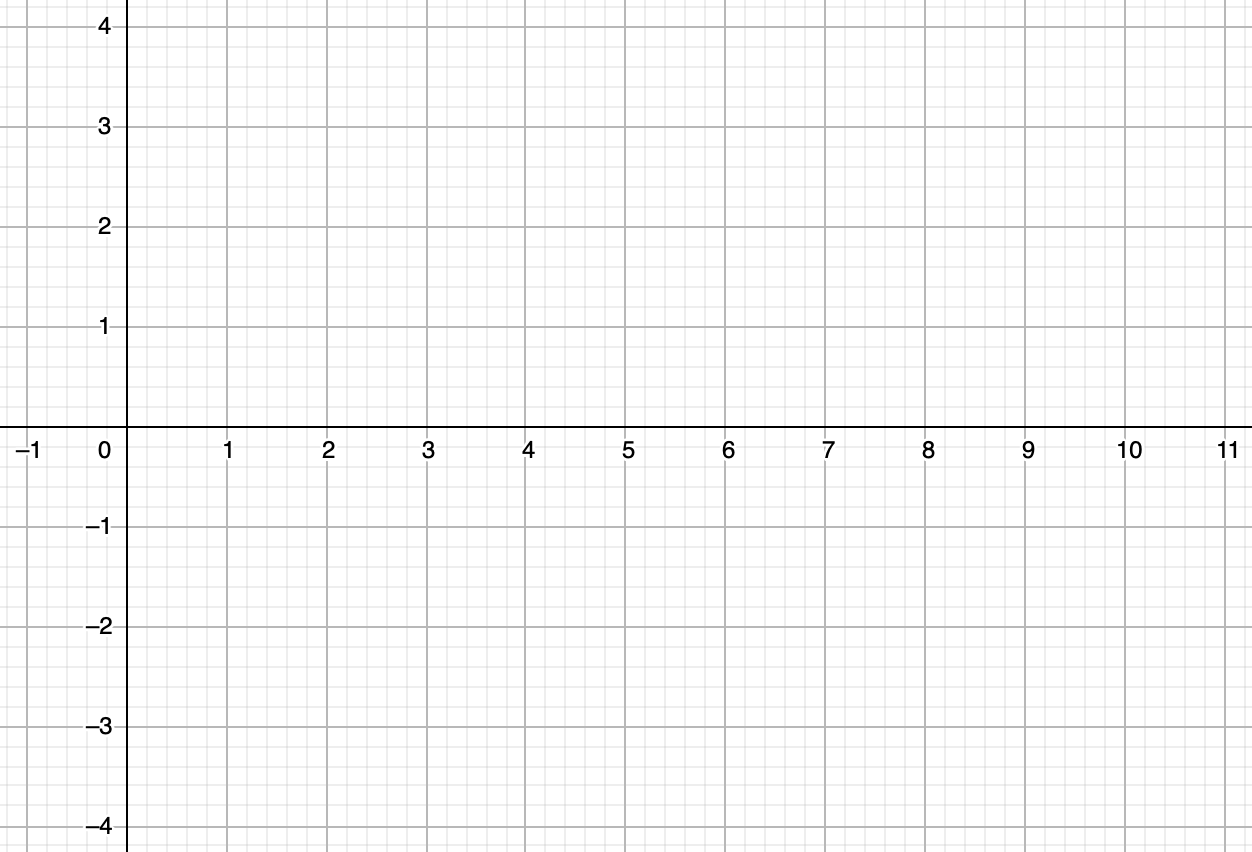
\includegraphics{images/CP-3-LT2-grid.png}} 
	\end{center}
	
	Let $F$ be an antiderivative of $f$ that satisfies $F(1) = -2$.
	
	\begin{enumerate}[leftmargin=0pt]
		\item On what intervals is $F$ increasing?  decreasing? neither?  why?
		
		\vfill
		
		\item On what intervals is $F$ concave up?  concave down?  neither?  why?
		
		\vfill
		
		\item Find the exact values of $F(2)$, $F(3)$, $F(5)$, $F(6)$, $F(8)$, and $F(10)$.  Write one sentence to explain briefly how you found these values.
		
		\vfill
		\vfill
		
		\item On the blank grid at right, sketch an accurate, labeled graph of $y = G(x)$.
		
	\end{enumerate}


\pagebreak
%%%%%%%%%%%%%%%%%%%%%%%%%%%%%%%%%%%%%%%%%%%%%%%%%%%%%%%
\section{Learning target I3, version 2}

Use integration by substitution and integration by parts to find antiderivatives. Decide which method to apply to a given integral.

\hrulefill

Evaluate each of the following integrals. For each one:
\begin{itemize}
	\item show all your work, including any new variables you use,
	\item and write one sentence that explains your choice of method and substitution.
\end{itemize}
Your process is even more important than your answer in each. Use the back of this paper if you need more room to explain your thinking.

\begin{enumerate}
	\item $\int 5x \sin(2x) \, dx$
			
	\vfill

	\item $\int e^x \cos(e^x) \, dx$

	\vfill

	\item $\int x^7 \ln(x) \, dx$
	\vfill
\end{enumerate}
%%%%%%%%%%%%%%%%%%%%%%%%%%%%%%%%%%%%%%%%%%%%%%%%%%%%%%%

\end{document}